% !TEX root = ../main.tex

\chapter{Stand der Technik}
%\chapter{Related Work}
\label{ch:relatedWork}

% Dieses Kapitel kann auch als Abschnitt im vorherigem Grundlagen Kapitel enthalten sein.
% Dies kann je nach Art der verwandten Arbeit und wie diese mit der aktuellen Arbeit verknüpft ist eine logischere Gliederung darstellen.
% This chapter can alternatively be a section of the background chapter. Depending on the relations between the actual and the related work,
% it can be a more intuitive, logic and consistent structuring to mention the related work in the previous chapter.

% Kurz vorstellen was es noch in dem Gebiet gibt und worin sich diese Arbeit davon unterscheidet
% Short presentation/summary of what has been done already in the research area and how it differs from the current thesis.
In diesem Kapitel werden die bestehenden Tools zum Spezifizieren von Architekturen im Bereich der Fahrzeugindustrie sowie die von ihnen verwendeten Verfahren zur Architekturvalidierung vorgestellt. Dies ermöglicht ein besseres Verständnis für den Beitrag, den die Abschlussarbeit leistet.

\section{Etablierte Tools und Plattformen}
Um die zunehmende Komplexität der \glspl{eea} in modernen Fahrzeugen mit Blick auf autonome Fahrfunktionen und Fahrassistenzsystemen zu bewältigen, wird aktiv an Software gearbeitet, die es Entwicklern und Ingenieuren ermöglicht, funktionale, softwarebezogene und \glspl{eea} zu modellieren bzw. zu spezifizieren \cite{askaripoor2022architecture} \cite{schauffele2016architectural}. Im folgenden werden die Tools PREEvision und Simulink + System Composer, die als Industriestandard gelten, und Capella als kostenlose Alternative analysiert.


\subsection{Vector PREEvision}
PREEvision ist ein kommerzielles, modellbasiertes Tool zur Entwicklung und Optimierung verteilter, eingebetteter Systeme in der Automobilindustrie. Das Hauptziel des Tools ist es, die zunehmende Komplexität der \glspl{eea} innerhalb der \glspl{sdv} beherrschbar zu halten \cite{askaripoor2022architecture}. Das  Tool richtet sich dabei an die weit akzeptierten Automobilstandards wie \gls{autosar} RIF/ReqIF\footnote{Requirements Interchange Format: www.automotive-his.de/rif}, KBL\footnote{Kabelbaumliste: www.vda.de
} und VEC\footnote{Vehicle Electric Container: www.vda.de} \cite{schauffele2016architectural}. Es werden außerdem die drei System-Engineering-Prinzipien unterstützt: Abstraktion (Implementationsaspekte auf eine konzeptionellere Ebene abstrahieren), Dekomposition (System kann in jeder Schicht hierarchisch zerlegt werden), Wiederverwendung (Komponenten und Modelle können von verschiedensten Produktlinien und Varianten verwendet werden) \cite{schauffele2016architectural}.

\begin{figure}[h!]
  \centering
  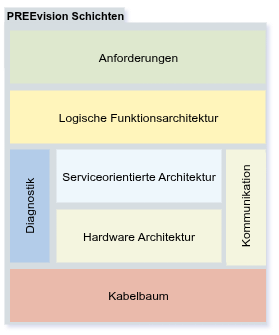
\includegraphics[width=0.5\textwidth]{figures/PREEVISION_LAYER.drawio.png}
  \caption{Schematische PREEvision Schichtenarchitektur. (Nachzeichnung von \cite{Vec23})}
  \label{fig:preevision_schicht}
\end{figure}

Der Schwerpunkt von PREEvision ist jedoch, die auf Abbildung~\ref{fig:preevision_schicht} dargestellte Schichtenarchitektur. Die Abbildung zeigt den Weg von der abstrakten Anforderungsebene zur konkreten Implementierung. Ausgehend von den Anforderungen wird eine Logische Funktionsarchitektur entworfen, die dann in eine \gls{soa} und eine Hardware Architektur überführt wird, bis hin zum physischen Kabelbaum. Dieser durchgängige Ansatz stellt sicher, dass alle Aspekte des Systems, inklusive Diagnostik und Kommunikation, miteinander verbunden sind (Single-Source-of-Truth) \cite{schauffele2016architectural}.


\subsection{Mathworks Simulink + System Composer}
Simulink und System Composer sind kommerzielle Tools, die eng miteinander integriert sind, um \gls{mbse} zu unterstützen \cite{watkins2020system}.
Während System Composer für die Modellierung und  Analyse der statischen System- und Softwarearchitektur verwendet wird, liegt der Fokus von Simulink in der Simulation des dynamischen Verhaltens dieser Architekturen. Dieses Zusammenspiel ermöglicht einen Übergang von dem reinen Architekturentwurf zu dem konkreten, ausführbaren Designmodell \cite{chatterjee2020applications}.

\begin{figure}[h!]
  \centering
  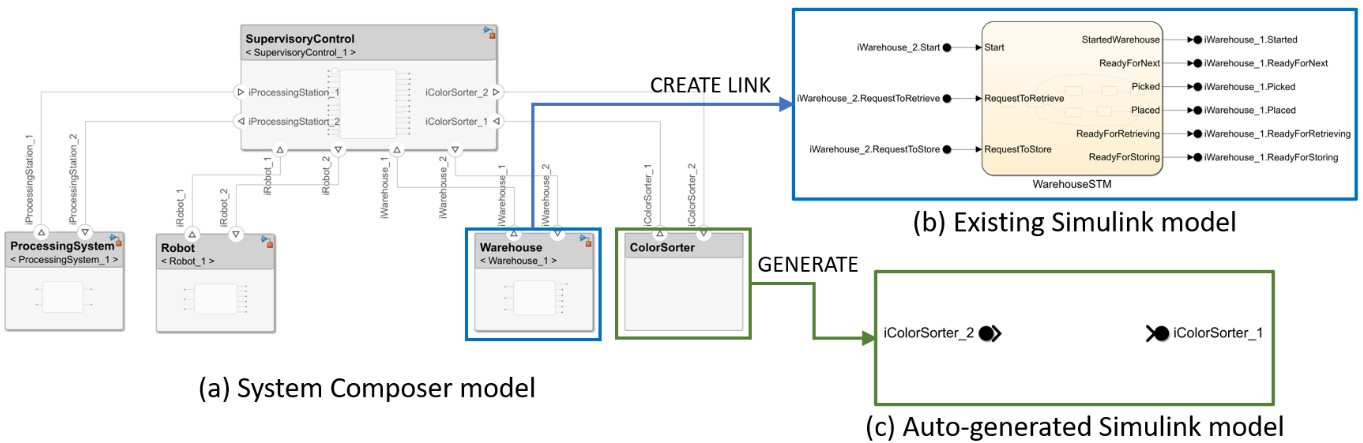
\includegraphics[width=\textwidth]{figures/03StandDerTechnik/Simulink_System_Composer.png}
  \caption{Verknüpfung einer System Composer Architektur mit einem Simulink Verhaltensmodell. (Entnommen aus \cite{chatterjee2020applications})}
  \label{fig:simulink_system_composer}
\end{figure}

Wie diese enge Integration praktisch umgesetzt wird, ist in Abbildung~\ref{fig:simulink_system_composer} zu sehen: Eine in System Composer entworfene Architekturkomponente wird direkt mit einem detaillierten Verhaltensmodell in Simulink verknüpft. Der diesem Vorgehen zugrundeliegende Arbeitsablauf folgt dem V-Modell\footnote{}, bei dem das Systemverhalten phasenweise modelliert und validiert wird \cite{The24}. Um komplexe und Verhaltensweisen modellieren zu können, werden spezielle Tools innerhalb von Simulink genutzt \cite{chatterjee2020applications}:

Stateflow dient zur Modellierung der Logik von Systemen mittels Zustandsautomaten, Flussdiagrammen oder Wahrheitstafeln. Es wird insbesondere für die übergeordnete Steuerung (Supervisory Control) und dem Fehlermanagement genutzt \cite{chatterjee2020applications}. Die Fähigkeit, ereignisdiskrete Systeme zu modellieren oder analysieren, wird durch SimEvents ermöglicht. Mithilfe von nachrichten- und entitätenbasierten Konzepten können Leistungsmerkmale, wie der Durchsatz oder die Latenz optimiert werden \cite{chatterjee2020applications}.

Wie auch bei PREEvision, unterstützt dieser gesamte Ansatz die zentralen System-Engineering Prinzipien: Abstraktion, Dekomposition und Wiederverwendung \cite{The24}.

\subsection{Eclipse Capella}
Capella ist ein nicht-kommerzielles Modellierungstool, das auf der Engineering-Methode ARCADIA\footnote{ARChitecture Analysis and Design Integrated Approach} basiert \cite{roques2016mbse}. Diese umfassende Methodik gibt einen klaren, schrittweisen Konstruktionsprozess vor, der den Anwender von der Bedarfsanalyse bis zum detaillierten Architektur-Design führt \cite{let24}.

\begin{figure}[h!]
  \centering
  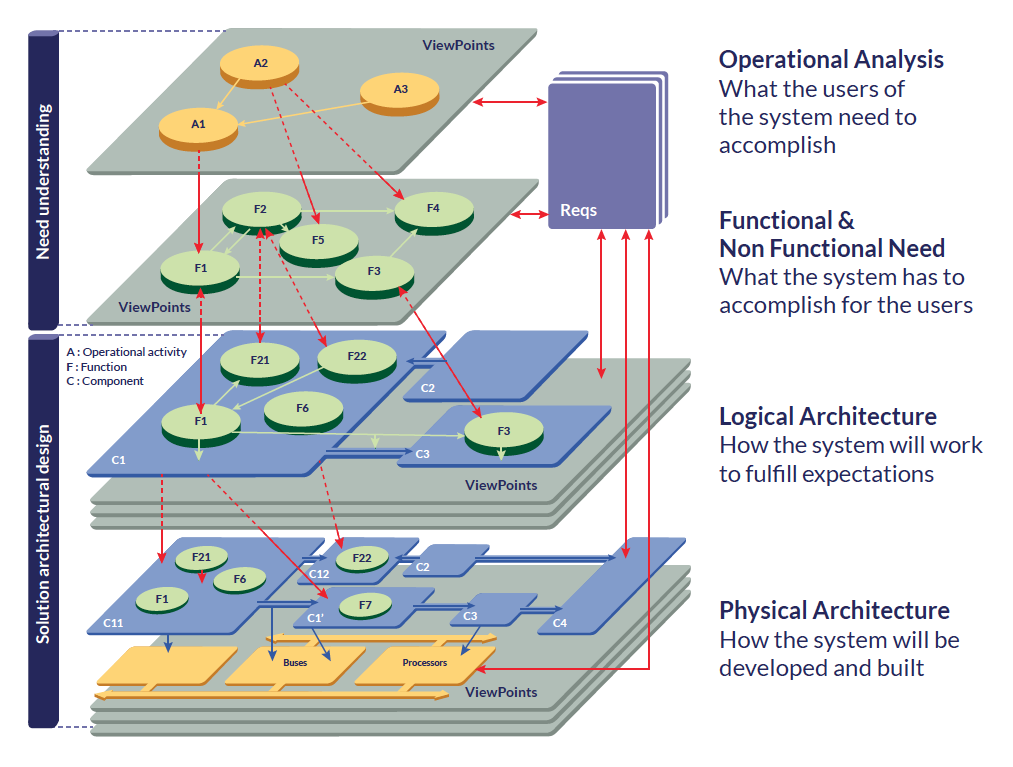
\includegraphics[width=.7\textwidth]{figures/03StandDerTechnik/phases_arcadia.png}
  \caption{Das Arcadia-Vorgehensmodell in Capella als vier übereinander gestapelte Architekturebenen (Entnommen aus \cite{let24})}
  \label{fig:capella_modell}
\end{figure}

Die Abbildung~\ref{fig:capella_modell} zeigt die vier Konstruktionsphasen von Arcadia. Der Prozess beginnt mit der Betriebsanalyse, in der untersucht wird, was die Erwartungen, Anwendungsbedingungen, Integrations-, Verifikations- und Validierungsvorraussetzungen des Endnutzer sind. Darauf aufbauend folgt die Funktionale \& Nicht-Funktionale Bedarfsanalyse, in der die Systemfunktionen und nicht-funktionalen Anforderungen abgeleitet werden.

Bei Arcadia haben Bedarfsanalyse und Modellierung, Architekturentwicklung und -validierung sowie Anforderungsanalyse die gleiche Wichtigkeit. Wobei die Anforderungen gegen eine frühe Version des Architekturmodells auf Robustheit und Machbarkeit geprüft werden.

Nachdem System, Hardware und Software modelliert wurden, wird eine logische Architektur entwickelt. Dabei wird nach einem Kompromiss zwischen Entwurfsfaktoren, (nicht-funktionalen) Bedingungen und Ansichten gesucht. Jede Ansicht beschäftigt sich mit bestimmten Aspekten wie funktionale Konsistenz, Schnittstellen, Leistung, Echtzeit, Sicherheit, Integration, Wiederverwendung, Kosten und Risiko.

Abschließend beschreibt die physische Architektur die Umsetzung auf konkrete Hardware- und Softwarekomponenten und sichert durch die Trennung der Aspekte, Schichtenarchitekturen und standardisierte Interaktionsmuster eine effiziente, sichere Entwicklung und Integration, Verifizierung \& Validierung, Qualifizierungsaktivitäten \cite{let24}.

Während Arcadia die komplette linke Seite des V-Modells abdeckt, deckt das Produktlebenszyklusmanagement (PLM) die rechte Seite des Modells ab und garantiert somit eine vollständige Umsetzung des V-Modells \cite{2024arcadia}.

\section{Validierungsverfahren im Detail}

Ein zentraler Aspekt moderner Architekturtools ist die Fähigkeit, entworfene Modelle zu validieren und deren Qualität sicherzustellen. Die in dieser Arbeit analysierten Tools verfolgen dabei unterschiedliche Ansätze und decken verschiedene Bereiche der Architekturvalidierung ab, die in Tabelle~\ref{tab:validierungsvergleich} vergleichend dargestellt werden.

\begin{table}[h!]
  \centering
  \footnotesize % Kleinere Schriftgröße für maximale Kompaktheit
  \begin{tabularx}{\textwidth}{X c c c}
    \toprule
    \textbf{Validierungsart}          & \textbf{PREEvision} & \textbf{Capella} & \textbf{Simulink} \\
    \midrule
    \multicolumn{4}{l}{\textit{Modell-Integrität \& Konsistenz}}                                   \\
    Inkonsistenz/Vollständigkeit      & \checkmark          & \checkmark       & \checkmark        \\
    Nachverfolgbarkeit                & \checkmark          & \checkmark       & \checkmark        \\
    Ebenenübergreifende Realisierung  & \checkmark          & \checkmark       &                   \\
    \midrule
    \multicolumn{4}{l}{\textit{Anforderungs- \& Design-Validierung}}                               \\
    Validierung gegen Anforderungen   & \checkmark          & \checkmark       & \checkmark        \\
    Analyse von Designalternativen    & \checkmark          & \checkmark       & \checkmark        \\
    \midrule
    \multicolumn{4}{l}{\textit{Quantitative Analysen \& Metriken}}                                 \\
    Performance-Analyse               & \checkmark          & \checkmark       & \checkmark        \\
    Netzwerk- und Ressourcen-Metriken & \checkmark          &                  &                   \\
    Statische Analyse                 &                     & \checkmark       & \checkmark        \\
    \midrule
    \multicolumn{4}{l}{\textit{Sicherheits- \& Zuverlässigkeitsanalysen}}                          \\
    Sicherheitsanalysen               & \checkmark          & \checkmark       &                   \\
    Fehlerfortpflanzungsanalyse       &                     & \checkmark       &                   \\
    \midrule
    \multicolumn{4}{l}{\textit{Verhaltensbasierte Validierung}}                                    \\
    Dynamische Simulation             &                     &                  & \checkmark        \\
    \midrule
    \multicolumn{4}{l}{\textit{Versions-Validierung}}                                              \\
    Prüfung von Modellversionen       & \checkmark          & \checkmark       & \checkmark        \\
    \bottomrule
  \end{tabularx}
  \caption{Auflistung der Architekturvalidierungen nach Tool}
  \label{tab:validierungsvergleich}
\end{table}

Eine kurze Analyse der ausgewählten Tools zeigt, dass jedes von ihnen seine spezifischen Stärken in unterschiedlichen Bereichen der Architekturvalidierung besitzt. Während PREEvision bei E/E-spezifischen Metriken wie Netzwerk- und Ressourcenmetriken sowie Sicherheitsanalysen dominiert \cite{schauffele2016architectural}, liegen die Stärken von Capella in der Sicherstellung der Architekturkonsistenz über mehrere Ebenen hinweg \cite{roques2016mbse}. Als einziges Tool bietet Simulink zudem die Möglichkeit zur dynamischen Validierung des Systemverhaltens mittels ausführbarer Simulation \cite{The24}.

In der Praxis ergibt sich durch diese hohe Spezialisierung eine zentrale Herausforderung: Keines der Tools deckt alle notwendigen Validierungsverfahren ab. Darüber hinaus sind diese Systeme meist geschlossene Plattformen. Die Anbindung neuer oder unternehmensspezifischer Validierungsalgorithmen, die vom Hersteller nicht vorgesehen sind, ist häufig gar nicht oder nur mit erheblichem Aufwand möglich. Es fehlt an flexiblen und offenen Schnittstellen zur Integration externer Algorithmen.

\break
Genau an dieser Stelle setzt die Bachelorarbeit an. Ziel dieser Arbeit ist es, das generische, webbasierte \textit{ArchitekturTool} um ein Framework zur automatisierten Architekturvalidierung zu erweitern. Durch die Implementierung einer offenen \gls{api}-Schnittstelle soll die bestehende Lücke hinsichtlich mangelnder Flexibilität geschlossen und die einfache Anbindung beliebiger Validierungsalgorithmen ermöglicht werden.
